\let\negmedspace\undefined
\let\negthickspace\undefined
\documentclass[journal,12pt,onecolumn]{IEEEtran}
\usepackage{cite}
\usepackage{amsmath,amssymb,amsfonts,amsthm}
\usepackage{algorithmic}
\usepackage{graphicx}
\usepackage{textcomp}
\usepackage{xcolor}
\usepackage{txfonts}
\usepackage{listings}
\usepackage{enumitem}
\usepackage{mathtools}
\usepackage{gensymb}
\usepackage{comment}
\usepackage[breaklinks=true]{hyperref}
\usepackage{tkz-euclide} 
\usepackage{gvv}                                        
%\def\inputGnumericTable{}                                 
\usepackage[latin1]{inputenc}     
\usepackage{xparse}
\usepackage{color}                                            
\usepackage{array}                                            
\usepackage{longtable}                                       
\usepackage{calc}                                             
\usepackage{multirow}
\usepackage{multicol}
\usepackage{hhline}                                           
\usepackage{ifthen}                                           
\usepackage{lscape}
\usepackage{tabularx}
\usepackage{float}
\newtheorem{theorem}{Theorem}[section]
\newtheorem{problem}{Problem}
\newtheorem{proposition}{Proposition}[section]
\newtheorem{lemma}{Lemma}[section]
\newtheorem{corollary}[theorem]{Corollary}
\newtheorem{example}{Example}[section]
\newtheorem{definition}[problem]{Definition}
\newcommand{\BEQA}{\begin{eqnarray}}
\newcommand{\EEQA}{\end{eqnarray}}
\newcommand{\define}{\stackrel{\triangle}{=}}
\theoremstyle{remark}
\newtheorem{rem}{Remark}
% Marks the beginning of the document
\begin{document}
\title{PI : PRODUCTION AND INDUSTRIAL ENGINEERING}
\author{AI25BTECH11034 - Sujal Chauhan}
\maketitle
\renewcommand{\thefigure}{\theenumi}
\renewcommand{\thetable}{\theenumi}
\textbf{Q.1 -- Q.5 carry one mark each.}

\begin{enumerate}

% Q.1
\item If I were you , I \underline{\hspace{1.5cm}} that laptop. It's much too expensive.  
\hfill{(GATE 2016)}

\begin{enumerate}
    \item won't buy
    \item sha't buy
    \item wouldn't buy
    \item would buy
\end{enumerate}
\vspace{1cm}

% Q.2
\item He \underline{turned a deaf ear} to my request.  

What does the underlined phrasal verb mean?  
\hfill{(GATE 2016)}

\begin{enumerate}
    \item ignored
    \item appreciated
    \item twisted
    \item returned
\end{enumerate}
\vspace{1cm}

% Q.3
\item Choose the most appropriate set of words from the options given below to complete the following sentence.  

\underline{\hspace{1.5cm}} \underline{\hspace{1.5cm}} is a will, \underline{\hspace{1.5cm}} is a way.  
\hfill{(GATE 2016)}

\begin{enumerate}
    \item Wear, there, their
    \item Were, their, there
    \item Where, there, there
    \item Where, their, their
\end{enumerate}
\vspace{1cm}

% Q.4
\item $(x\% \text{ of } y) + (y\% \text{ of } x)$ is equivalent to \underline{\hspace{2cm}}  
\hfill{(GATE 2016)}

\begin{enumerate}
    \item $2\%$ of $xy$
    \item $2\%$ of $(xy/100)$
    \item $xy\%$ of $100$
    \item $100\%$ of $xy$
\end{enumerate}
\vspace{1cm}

% Q.5
\item The sum of the digits of a two digit number is $12$. If the new number formed by reversing the digits is greater than the original number by $54$, find the original number.  
\hfill{(GATE 2016)}

\begin{enumerate}
    \item 39
    \item 57
    \item 66
    \item 93
\end{enumerate}
\vspace{1cm}

\textbf{Q.6 -- Q.10 carry two marks each.}



% Q.6
\item Two finance companies, P and Q, declared fixed annual rates of interest on the amounts invested with them. The rates of interest offered by these companies may differ from year to year. Year-wise annual rates of interest offered by these companies are shown by the line graph provided below.  

\begin{figure}[h!]
    \centering
    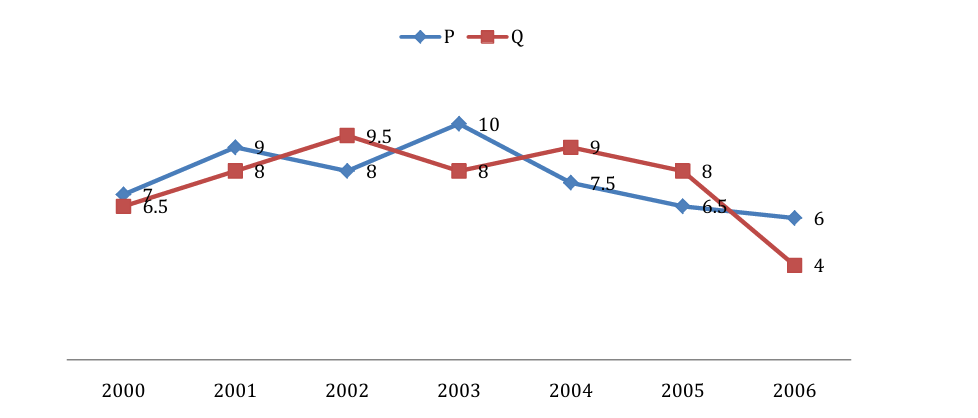
\includegraphics[width=0.7\textwidth]{GATE-PI-2016/4-GA-GATE-2016.png} % 
\end{figure}

If the amounts invested in the companies, P and Q, in 2006 are in the ratio 8:9, then the amounts received after one year as interests from companies P and Q would be in the ratio:  
\hfill{(GATE 2016)}

\begin{enumerate}
    \item 2:3
    \item 3:4
    \item 6:7
    \item 4:3
\end{enumerate}
\vspace{1cm}

% Q.7
\item Today, we consider Ashoka as a great ruler because of the copious evidence he left behind in the form of stone carved edicts. Historians tend to correlate greatness of a king at his time with the availability of evidence today.  

Which of the following can be logically inferred from the above sentences?  
\hfill{(GATE 2016)}

\begin{enumerate}
    \item Emperors who do not leave significant sculpted evidence are completely forgotten.
    \item Ashoka produced stone carved edicts to ensure that later historians will respect him.
    \item Statues of kings are a reminder of their greatness.
    \item A king's greatness, as we know him today, is interepreted by historians.
\end{enumerate}
\vspace{1cm}

% Q.8
\item Fact 1: Humans are mammals. \\
Fact 2: Some humans are engineers. \\
Fact 3: Engineers build houses.  

If the above statements are facts, which of the following can be logically inferred?  
\hfill{(GATE 2016)}

\begin{enumerate}
    \item II only.
    \item III only.
    \item I, II and III.
    \item I only.
\end{enumerate}
\vspace{1cm}

% Q.9
\item A square pyramid has a base perimeter $x$, and the slant height is half of the perimeter. What is the lateral surface area of the pyramid?  
\hfill{(GATE 2016)}

\begin{enumerate}
    \item $x^2$
    \item $0.75\,x^2$
    \item $0.50\,x^2$
    \item $0.25\,x^2$
\end{enumerate}
\vspace{1cm}

% Q.10
\item Ananth takes 6 hours and Bharath takes 4 hours to read a book. Both started reading copies of the book at the same time. After how many hours is the number of pages to be read by Ananth, twice that to be read by Bharath? Assume Ananth and Bharath read all the pages with constant pace.  
\hfill{(GATE 2016)}

\begin{enumerate}
    \item 1
    \item 2
    \item 3
    \item 4
\end{enumerate}
\vspace{10cm}
\begin{center}
 \textbf{\Large END OF QUESTION PAPER}   
\end{center}
\newpage



\end{enumerate}


\begin{center}
    {\Large \textbf{Q.1 -- Q.25 carry one mark each.}}
\end{center}

\begin{enumerate}

% Q.1
\item The eigenvalues of the matrix
\[
\myvec{0 & 1 \\ -1 & 0}
\]
are  
\hfill{(GATE 2016)}

\begin{multicols}{4}
\begin{enumerate}
    \item $i$ and $-i$
    \item $1$ and $-1$
    \item $0$ and $1$
    \item $0$ and $-1$
\end{enumerate}
\end{multicols}
\vspace{1cm}

% Q.2
\item The number of solutions of the simultaneous algebraic equations 
\[
y = 3x+3 \quad \text{and} \quad y=3x+5
\]
is  
\hfill{(GATE 2016)}

\begin{multicols}{4}
\begin{enumerate}
    \item zero
    \item 1
    \item 2
    \item infinite
\end{enumerate}
\end{multicols}
\vspace{1cm}

% Q.3
\item At $x=0$, the function
\[
f(x) = \left|\frac{\sin \frac{2\pi x}{L}}{x}\right|, \quad (-\infty < x < \infty, \; L>0)
\]
is  
\hfill{(GATE 2016)}

\begin{enumerate}
    \item continuous and differentiable.
    \item not continuous and not differentiable.
    \item not continuous but differentiable.
    \item continuous but not differentiable.
\end{enumerate}
\vspace{1cm}

% Q.4
\item For the two functions 
\[
f(x,y) = x^3 - 3xy^2 \quad \text{and} \quad g(x,y) = 3x^2y - y^3
\]
which one of the following options is correct?  
\hfill{(GATE 2016)}

\begin{multicols}{4}
\begin{enumerate}
    \item $\dfrac{\partial f}{\partial x} = \dfrac{\partial g}{\partial y}$
    \item $\dfrac{\partial f}{\partial x} = -\dfrac{\partial g}{\partial y}$
    \item $\dfrac{\partial f}{\partial y} = -\dfrac{\partial g}{\partial x}$
    \item $\dfrac{\partial f}{\partial y} = \dfrac{\partial g}{\partial x}$
\end{enumerate}
\end{multicols}
\vspace{1cm}

% Q.5
\item The function 
\[
f(z) = \frac{z^2+1}{z^2+4}
\]
is singular at  
\hfill{(GATE 2016)}

\begin{multicols}{4}
\begin{enumerate}
    \item $z=\pm 2$
    \item $z=\pm 1$
    \item $z=\pm i$
    \item $z=\pm 2i$
\end{enumerate}
\end{multicols}
\vspace{1cm}
\newpage

% Q.6
\item A fair coin is tossed $N$ times. The probability that head does not turn up in any of the tosses is  
\hfill{(GATE 2016)}

\begin{multicols}{4}
\begin{enumerate}
    \item $\left(\tfrac{1}{2}\right)^{N-1}$
    \item $1 - \left(\tfrac{1}{2}\right)^{N-1}$
    \item $\left(\tfrac{1}{2}\right)^N$
    \item $1 - \left(\tfrac{1}{2}\right)^N$
\end{enumerate}
\end{multicols}
\vspace{1cm}
% Q.7
\item A normal random variable $X$ has the following probability density function
\[
f_X(x) = \frac{1}{\sqrt{8\pi}} e^{-\frac{(x-1)^2}{8}}, \quad -\infty < x < \infty
\]
Then $\int_{1}^{\infty} f_X(x)\,dx =$  
\hfill{(GATE 2016)}

\begin{multicols}{4}
\begin{enumerate}
    \item $0$
    \item $\tfrac{1}{2}$
    \item $1 - \tfrac{1}{e}$
    \item $1$
\end{enumerate}
\end{multicols}
\vspace{1cm}

% Q.8
\item The elastic modulus of a rigid perfectly plastic solid is  
\hfill{(GATE 2016)}

\begin{multicols}{4}
\begin{enumerate}
    \item $0$
    \item $1$
    \item $100$
    \item infinity
\end{enumerate}
\end{multicols}
\vspace{1cm}

% Q.9
\item Consider the following statements:  

(P) Hardness is the resistance of a material to indentation.  
(Q) Elastic modulus is a measure of ductility.  
(R) Deflection depends on stiffness.  
(S) The total area under the stress-strain curve is a measure of resilience.  

Among the above statements, the correct ones are  
\hfill{(GATE 2016)}

\begin{multicols}{4}
\begin{enumerate}
    \item P and Q only.
    \item Q and S only.
    \item P and R only.
    \item R and S only.
\end{enumerate}
\end{multicols}
\vspace{1cm}
\newpage
% Q.10
\item A beam is subjected to an inclined concentrated load as shown in the figure below. 
Neglect the weight of the beam.  
\hfill{(GATE 2016)}
\begin{figure}[H]
    \centering
    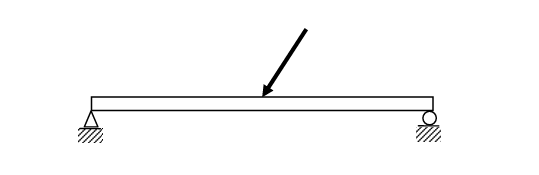
\includegraphics[width=0.5\linewidth]{GATE-PI-2016/10-GATE-PI-2016.png}
    \caption{}
    \label{q10}
\end{figure}

The correct Free Body Diagram of the beam is  

\begin{figure}[H]
    \centering
    \begin{minipage}{0.45\linewidth}
        \centering
        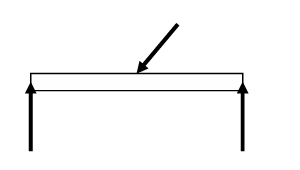
\includegraphics[width=0.7\linewidth]{GATE-PI-2016/10A-GATE-PI-2016.png}
        \caption{a)}
        \label{q10a}
    \end{minipage}\hfill
    \begin{minipage}{0.45\linewidth}
        \centering
        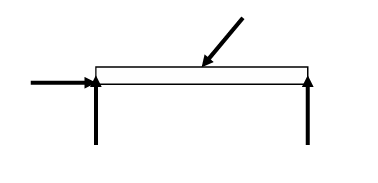
\includegraphics[width=0.7\linewidth]{GATE-PI-2016/10B-GATE-PI-2016.png}
          \caption{b)}
        \label{q10b}
    \end{minipage}

    \vspace{0.5cm}

    \begin{minipage}{0.45\linewidth}
        \centering
        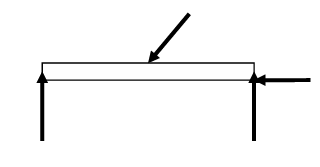
\includegraphics[width=0.7\linewidth]{GATE-PI-2016/10C-GATE-PI-2016.png}
         \caption{c)}
        \label{q10c}
    \end{minipage}\hfill
    \begin{minipage}{0.45\linewidth}
        \centering
        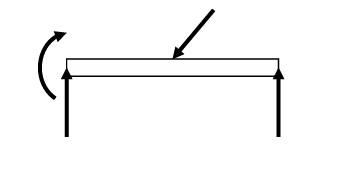
\includegraphics[width=0.7\linewidth]{GATE-PI-2016/10D-GATE-PI-2016.png}
        \caption*{d)}
        \label{q10d}
    \end{minipage}
\end{figure}

\vspace{1cm}
\newpage
% Q.11
\item Consider a circular cam with a flat face follower as shown in the figure below. 
The cam is rotated in the plane of the paper about point P lying 5 mm away from its center. 
The radius of the cam is 20 mm. The distance (in mm) between the highest and the lowest 
positions of the flat face follower is \hfill{(GATE 2016)} 

\begin{figure}[H]
    \centering
    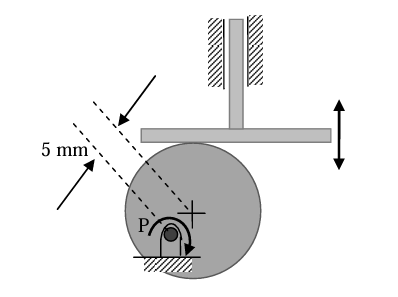
\includegraphics[width=0.45\linewidth]{GATE-PI-2016/11-GATE-PI-2016.png}
    \caption{}
    \label{q11}
\end{figure}

\begin{multicols}{4}
  \begin{enumerate}
      \item 5
      \item 10
      \item 40
      \item 45
  \end{enumerate}  
\end{multicols}

\vspace{1cm}

% Q.12
\item A vertical cylindrical tank of 1 m diameter is filled with water up to a height of 5 m from its bottom. 
Top surface of water is exposed to atmosphere. A hole of $5 \, \text{mm}^2$ area forms at the bottom of the tank. 
Considering the coefficient of discharge of the hole to be unity and the acceleration due to gravity to be $10 \, \text{m/s}^2$, 
the rate of leakage of water (in litre/min) through the hole from the tank to the atmosphere, under the given conditions, is \underline{\hspace{2cm}}.  \hfill{(GATE 2016)}

\vspace{1cm}


\newpage
% Q.13
\item The figure below shows an air standard Diesel cycle in $p$-$V$ diagram. 
The cut-off ratio is given by:  \hfill{(GATE 2016)}

\begin{figure}[H]
    \centering
    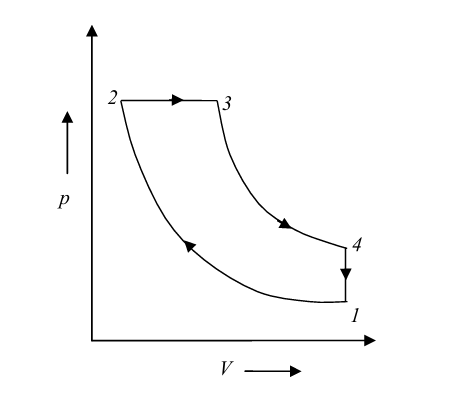
\includegraphics[width=0.45\linewidth]{GATE-PI-2016/13-GATE-PI-2016.png}
    \caption{}
    \label{q13}
\end{figure}

\begin{multicols}{4}
\begin{enumerate}
    \item $\dfrac{V_3}{V_1}$
    \item $\dfrac{V_2}{V_1}$
    \item $\dfrac{V_3}{V_2}$
    \item $\dfrac{V_1}{V_3}$
\end{enumerate}
\end{multicols}

\vspace{0.5cm}

% Q.14
\item The ratio of press force required to punch a square hole of 30 mm side in a 1 mm thick aluminium sheet 
to that needed to punch a square hole of 60 mm side in a 2 mm thick aluminium sheet is \underline{\hspace{2cm}}. \hfill{(GATE 2016)} 

\vspace{0.5cm}

% Q.15
\item Which one of the following is a natural polymer? \hfill{(GATE 2016)} 

\begin{multicols}{4}
\begin{enumerate}
    \item Cellulose
    \item Nylon
    \item Polyester
    \item Polyvinyl chloride
\end{enumerate}
\end{multicols}

\vspace{0.5cm}

% Q.16
\item In powder metallurgy, sintering of the component  \hfill{(GATE 2016)}

\begin{multicols}{2}
\begin{enumerate}
    \item increases density and reduces ductility.
    \item increases porosity and reduces density.
    \item increases density and reduces porosity.
    \item increases porosity and reduces brittleness.
\end{enumerate}
\end{multicols}

\vspace{0.5cm}

% Q.17
\item A single point right handed turning tool is used for straight turning. 
The feed is 0.25 mm/rev and the uncut chip thickness is found to be 0.25 mm. 
The inclination angle of the main cutting edge is $10^\circ$. 
The back rake angle (in degrees) is \underline{\hspace{2cm}}.  \hfill{(GATE 2016)}


% Q.18
\item Consider the following statements:
\begin{enumerate}[label=(\Alph*)]
    \item Electrolyte is used in Electro-chemical machining.
    \item Electrolyte is used in Electrical discharge machining.
    \item Abrasive-slurry is used in Ultrasonic machining.
    \item Abrasive-slurry is used in Abrasive jet machining.
\end{enumerate}
Among the above statements, the correct ones are \hfill{(GATE 2016)}
\begin{multicols}{2}
\begin{enumerate}
    \item P and R only
    \item Q and S only
    \item Q, R and S only
    \item P and Q only
\end{enumerate}
\end{multicols}
\vspace{0.5cm}

% Q.19
\item Consider the following statements:
\begin{enumerate}[label=(\Alph*)]
    \item Computer aided process planning (CAPP) takes input from material requirement plan (MRP).
    \item Production flow analysis helps in work cell formation.
    \item Group technology takes input from choice of machining or cutting parameters.
\end{enumerate}
Among the above statements, the correct one(s) is (are)\hfill{(GATE 2016)}
\begin{multicols}{2}
\begin{enumerate}
    \item P only
    \item Q and R only
    \item P and R only
    \item Q only
\end{enumerate}
\end{multicols}
\vspace{0.5cm}

% Q.20
Among the above statements, the correct one(s) is (are)
\item The limits of a shaft designated as 100h5 are 100.000 mm and 100.014 mm. Similarly, the limits of a shaft designated as 100h8 are 100.000 mm and 100.055 mm. If a shaft is designated as 100h6, the fundamental deviation (in $\mu$m) for the same is \hfill{(GATE 2016)}
\begin{multicols}{4}
\begin{enumerate}
    \item $-22$
    \item zero
    \item $22$
    \item $24$
\end{enumerate}
\end{multicols}
\vspace{0.5cm}

% Q.21
\item The roughness profile of a surface is depicted below.\hfill{(GATE 2016)}
\begin{figure}[h!]
    \centering
    
    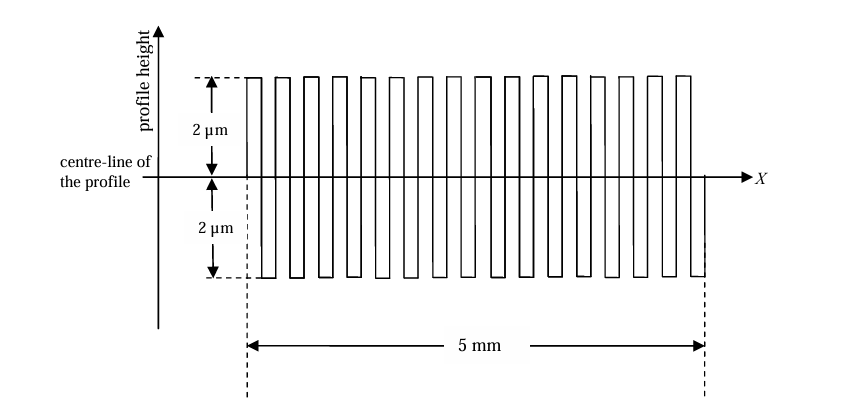
\includegraphics[width=0.6\textwidth]{GATE-PI-2016/21-GATE-PI-2016.png}
    \caption{}
    \label{q21}
\end{figure}
\\The surface roughness parameter $R_{a}$ (in $\mu$m) is \underline{\hspace{1cm}}.
\vspace{0.5cm}






% Q.22
\item The facility layout technique that uses relationship (REL) chart is  \hfill{(GATE 2016)}

\begin{multicols}{2}
\begin{enumerate}
    \item CRAFT.
    \item Travel chart.
    \item Partial Set Covering.
    \item ALDEP.
\end{enumerate}
\end{multicols}

\vspace{0.5cm}

% Q.23
\item For a random variable $X$, let $\bar{X}$ be the sample average. The sample size is $n$. 
The mean and the standard deviation of $X$ are $\mu$ and $\sigma$, respectively. 
The standard deviation of $\bar{X}$ is  \hfill{(GATE 2016)}

\begin{multicols}{2}
\begin{enumerate}
    \item $n\sigma$
    \item $\sigma$
    \item $\dfrac{\sigma}{n}$
    \item $\dfrac{\sigma}{\sqrt{n}}$
\end{enumerate}
\end{multicols}

\vspace{0.5cm}

% Q.24
\item $ST$ and $NT$ denote the standard time and the normal time, respectively, to complete a job.  \hfill{(GATE 2016)}
Allowance $= LL \times ST$, where $0 < LL < 1$. Which one of the following relationships is correct?  

\begin{multicols}{2}
\begin{enumerate}
    \item $ST = \dfrac{NT}{(1 - LL)}$
    \item $ST = NT (1 + LL)$
    \item $ST = \dfrac{NT}{(1 + LL)}$
    \item $ST = NT (1 - LL)$
\end{enumerate}
\end{multicols}

\vspace{0.5cm}

% Q.25
\item The throughput rate of a production system is 20 units per hour. 
The average flow time is 30 minutes and the cycle time is 3 minutes. 
The average inventory (in units) in the system is  \hfill{(GATE 2016)}

\begin{multicols}{2}
\begin{enumerate}
    \item 1.5
    \item 9
    \item 10
    \item 11.33
\end{enumerate}
\end{multicols}

\vspace{0.5cm}

% Q.26
\item The range of values of $k$ for which the function  
\[
f(x) = (k^2 - 4)x^2 + 6x^3 + 8x^4
\]  
has a local maxima at point $x = 0$ is  \hfill{(GATE 2016)}

\begin{multicols}{2}
\begin{enumerate}
    \item $k < -2 \ \text{or} \ k > 2$
    \item $k \leq -2 \ \text{or} \ k \geq 2$
    \item $-2 < k < 2$
    \item $-2 \leq k \leq 2$
\end{enumerate}
\end{multicols}

\vspace{0.5cm}

% Q.27
\item 

$\lim_{x \to 0} \left(\frac{e^{5x} - 1}{x}\right)^2 \ \ \text{is equal to} \ \underline{\hspace{2cm}}$
\vspace{0.5cm} \hfill{(GATE 2016)}
% Q.28
\item To solve the equation  
\[
2 \sin x = x
\]  
by Newtona Raphson method, the initial guess was chosen to be $x = 2.0$. 
Consider $x$ in radian only. The value of $x$ (in radian) obtained after one iteration will be closest to  \hfill{(GATE 2016)}

\begin{multicols}{2}
\begin{enumerate}
    \item $-8.101$
    \item $1.901$
    \item $2.099$
    \item $12.101$
\end{enumerate}
\end{multicols}

\vspace{0.5cm}

% Q.29
\item In linear gas tungsten arc welding of two plates of the same material, 
the peak temperature $T$ (in K) is given as  
\[
T = \frac{C_1 q}{\sqrt{\alpha v}}
\]  
where $q$ is the heat input per unit length (in J/m) of weld, $\alpha$ is the thermal diffusivity (in m$^2$/s) of the plate materials and $C_1$ is a constant independent of process parameters and material types. Two welding cases are given below.  

Case I: $V = 15 \, \text{V}, \ I = 200 \, \text{A}, \ v = 5 \, \text{mm/s}, \ k = 150 \, \text{W/mK}, \ \rho = 3000 \, \text{kg/m}^3, \ C = 900 \, \text{J/kgK}$  

Case II: $V = 15 \, \text{V}, \ I = 300 \, \text{A}, \ v = 10 \, \text{mm/s}, \ k = 50 \, \text{W/mK}, \ \rho = 8000 \, \text{kg/m}^3, \ C = 450 \, \text{J/kgK}$  

where, $V$ is welding voltage, $I$ is welding current, $v$ is welding speed, and $k, \rho, C$ refer to the thermal conductivity, the density and the specific heat of the plate materials, respectively. Consider that electrical energy is completely converted to thermal energy. All other conditions remain same.  

The ratio of the peak temperature in Case I to that in Case II is  \hfill{(GATE 2016)}

\begin{multicols}{2}
\begin{enumerate}
    \item $\dfrac{1}{3}$
    \item $\dfrac{1}{2}$
    \item $1$
    \item $2$
\end{enumerate}
\end{multicols}

\vspace{0.5cm}

% Q.30
\item A bar of rectangular cross-sectional area of $50 \, \text{mm}^2$ is pulled from both the sides by equal forces of $100 \, \text{N}$ as shown in the figure below.  
The shear stress (in MPa) along the plane making an angle $45^\circ$ with the axis, shown as a dashed line in the figure, is \underline{\hspace{2cm}}. \hfill{(GATE 2016)} 

\begin{figure}[h!]
    \centering
    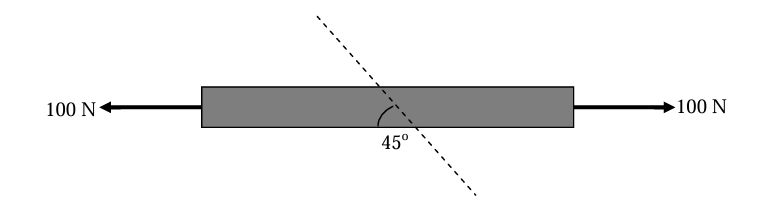
\includegraphics[width=0.45\textwidth]{GATE-PI-2016/30-GATE-PI-2016.png}
    \caption{}
    \label{q30}
\end{figure}

% Q.31
\item A $1~\text{m} \times 10~\text{mm} \times 10~\text{mm}$ cantilever beam is subjected to a uniformly distributed load per unit length of $100~\text{N/m}$ as shown in the figure below. The normal stress (in MPa) due to bending at point P is \underline{\hspace{2cm}}.\hfill{(GATE 2016)}
\begin{figure}[h!]
    \centering
    
    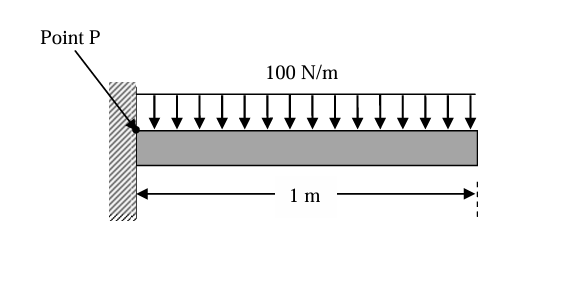
\includegraphics[width=0.55\textwidth]{GATE-PI-2016/31-GATE-PI-2016.png}
    \caption{}
    \label{q31}
\end{figure}
\vspace{0.5cm}

% Q.32
\item A thin-walled cylindrical pressure vessel of internal diameter $2~\text{m}$ is designed to withstand an internal pressure of $500~\text{kPa}$ (gauge). If the allowable normal stress at any point within the cylindrical portion of the vessel is $100~\text{MPa}$, the minimum thickness of the plate of the vessel (in mm) is \underline{\hspace{2cm}}.\hfill{(GATE 2016)}
\vspace{0.5cm}

% Q.33
\item An engine, connected with a flywheel, is designed to operate at an average angular speed of $800$~rpm. During operation of the engine, the maximum change in kinetic energy in a cycle is found to be $6240$~J. In order to keep the fluctuation of the angular speed within $\pm1\%$ of its average value, the moment of inertia (in kg-m$^{2}$) of the flywheel should be \underline{\hspace{2cm}}.\hfill{(GATE 2016)}
\vspace{0.5cm}
\newpage
% Q.34
\item A $2~\text{m} \times 2~\text{m}$ square opening in a vertical wall is covered with a metallic plate of the same dimensions as shown in the figure below. Consider the acceleration due to gravity to be $10.0~\text{m/s}^{2}$. The force (in kN) exerted by water on the plate is \underline{\hspace{2cm}}.\hfill{(GATE 2016)}
\begin{figure}[h!]
    \centering
    
    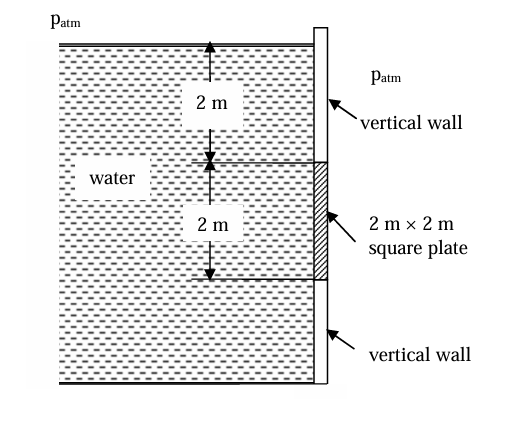
\includegraphics[width=0.45\textwidth]{GATE-PI-2016/34-GATE-PI-2016.png}
    \caption{}
    \label{q34}
    \end{figure}
\newpage
    % Q.35
\item An ideal gas of mass $m$ is contained in a rigid tank of volume $V$ at pressure $p$. During a reversible process its pressure reduces to $p_1$. Following statements are made regarding the process.\hfill{(GATE 2016)}

\begin{enumerate}[label=(\Alph*)]
    \item Heat is transferred from the gas.
    \item Work done by the gas is zero.
    \item Entropy of the gas remains constant.
    \item Entropy of the gas decreases.
\end{enumerate}

Among the above statements, the correct ones are
\begin{multicols}{2}
\begin{enumerate}
    \item P and R only
    \item P, Q and R only
    \item Q and R only
    \item P, Q and S only
\end{enumerate}
\end{multicols}
\vspace{0.5cm}

% Q.36
\item A long slender metallic rod of length $L$ is used as a fin. As shown in the figure below, the left end of the fin is kept at a constant temperature $t_b$. The fin loses heat by convection to the atmosphere which is at a temperature $t_a$ ($t_a < t_b$). Four options of temperature profiles are shown. Identify the correct option.\hfill{(GATE 2016)}

\begin{figure}[h!]
    \centering
    % Replace 'fin_main.png' with your actual image filename
    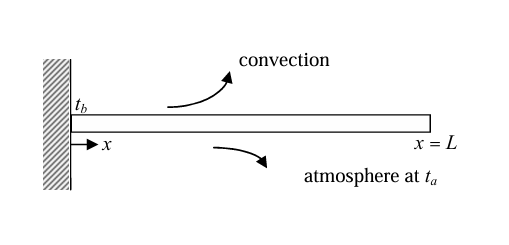
\includegraphics[width=0.55\textwidth]{GATE-PI-2016/36-GATE-PI-2016.png}
    \caption{Slender metallic rod used as a fin}
\end{figure}
\begin{enumerate}
    
\begin{multicols}{2}
    \item
    \begin{figure}[H]
        \centering
        % Replace 'temp_profile_A.png' with the actual option image filename
        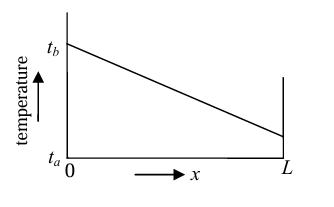
\includegraphics[width=0.18\textwidth]{GATE-PI-2016/36A-GATE-PI-2016.png}
         \caption{}
        \label{36a}
    \end{figure}

    \item
    \begin{figure}[H]
        \centering
        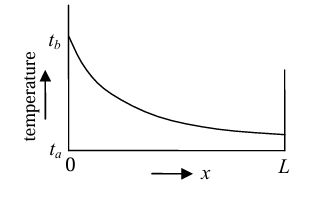
\includegraphics[width=0.18\textwidth]{GATE-PI-2016/36B-GATE-PI-2016.png}
         \caption{}
        \label{36b}
    \end{figure}

    \item
    \begin{figure}[H]
        \centering
        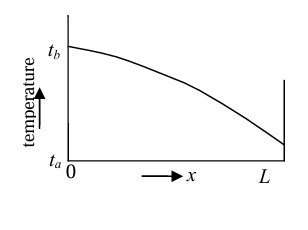
\includegraphics[width=0.18\textwidth]{GATE-PI-2016/36C-GATE-PI-2016.png}
         \caption{}
        \label{36c}
    \end{figure}

   \item
    \begin{figure}[H]
        \centering
        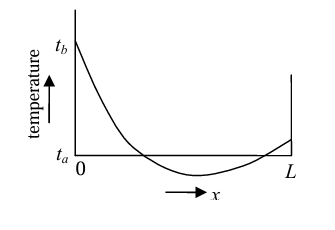
\includegraphics[width=0.18\textwidth]{GATE-PI-2016/36D-GATE-PI-2016.png}
        \caption{}
        \label{36d}
    \end{figure}
\end{multicols}
\end{enumerate}
\vspace{0.5cm}

\newpage
% Q.37
\item In a fully developed turbulent flow through a circular pipe, a head loss of $h_1$ is observed. The diameter of the pipe is increased by $10\%$ for the same flow rate and a head loss of $h_2$ is noted. Assume friction factor for both the cases of pipe flow is the same. The ratio of $\frac{h_2}{h_1}$ is closest to \hfill{(GATE 2016)}
\begin{multicols}{4}
\begin{enumerate}
    \item $0.34$
    \item $0.62$
    \item $0.87$
    \item $1.00$
\end{enumerate}
\end{multicols}
\vspace{0.5cm}

% Q.38
\item Two cast iron blocks P and Q, each of $500$~mm length, have the same cross-sectional area. Block P has rectangular cross-section of $100~\text{mm} \times 200~\text{mm}$. Block Q is of square cross-section. Both P and Q were cast under the same conditions with all their surfaces enclosed within the mould. The solidification time of a casting is proportional to the square of the ratio of its volume to its surface area. The ratio of solidification time of the block P to that of the block Q is \underline{\hspace{2cm}}.\hfill{(GATE 2016)}
\vspace{0.5cm}

% Q.39
\item A $300$~mm long copper wire of uniform cross-section is pulled in tension so that a maximum tensile stress of $270$~MPa is developed within the wire. The entire deformation of the wire remains linearly elastic. The elastic modulus of copper is $100$~GPa. The resultant elongation (in mm) is \underline{\hspace{2cm}}.\hfill{(GATE 2016)}
\vspace{0.5cm}

% Q.40
\item In a single-pass rolling operation, a $200$~mm wide metallic strip is rolled from a thickness $10$~mm to a thickness $6$~mm. The roll radius is $100$~mm and it rotates at $200$~rpm. The roll-strip contact length is a function of roll radius and, initial and final thickness of the strip. If the average flow stress in plane strain of the strip material in the roll gap is $500$~MPa, the roll separating force (in kN) is \underline{\hspace{2cm}}.\hfill{(GATE 2016)}
\vspace{0.5cm}

% Q.41
\item Two solid cylinders of equal diameter have different heights. They are compressed plastically by a pair of rigid dies to create the same percentage reduction in their respective heights. Consider that the die-workpiece interface friction is negligible. The ratio of the final diameter of the shorter cylinder to that of the longer cylinder is \underline{\hspace{2cm}}.\hfill{(GATE 2016)}
\vspace{0.5cm}

% Q.42
\item Two flat steel sheets, each of $2.5$~mm thickness, are being resistance spot welded using a current of $6000$~A and weld time of $0.2$~s. The contact resistance at the interface between the two sheets is $200~\mu\Omega$ and the specific energy to melt steel is $10 \times 10^6$~J/m$^3$. A spherical melt pool of diameter $4$~mm is formed at the interface due to the current flow. Consider that electrical energy is completely converted to thermal energy. The ratio of the heat used for melting to the total resistive heat generated is \underline{\hspace{2cm}}.\hfill{(GATE 2016)}
\vspace{0.5cm}

% Q.43
\item A cylindrical bar of $100$~mm diameter is orthogonally straight turned with cutting velocity, feed and depth of cut of $120$~m/min, $0.25$~mm/rev and $4$~mm, respectively. The specific cutting energy of the work material is $1 \times 10^6$~J/m$^3$. Neglect the contribution of feed force towards cutting power. The main or tangential cutting force (in N) is \underline{\hspace{2cm}}.\hfill{(GATE 2016)}
\vspace{0.5cm}
\newpage
% Q.44
\item A $60$~mm wide block of low carbon steel is face milled at a cutting speed of $120$~m/min, feed of $0.1$~mm/tooth and axial depth of cut of $4$~mm. A schematic representation of the face milling process is shown below. The diameter of the cutter is $120$~mm and it has $12$ cutting edges. The material removal rate (in mm$^3$/s) is \underline{\hspace{2cm}}.\hfill{(GATE 2016)}
\begin{figure}[h!]
    \centering
    % Replace 'face_milling.png' with your actual figure filename
    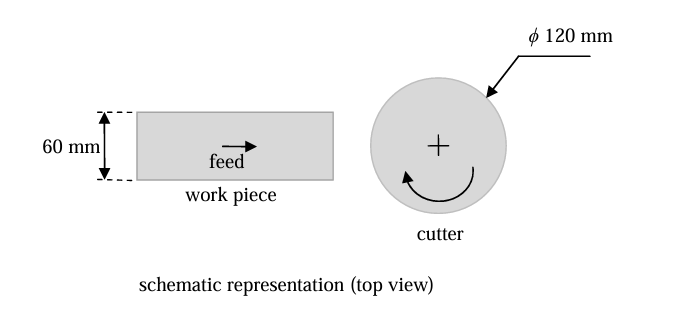
\includegraphics[width=0.56\textwidth]{GATE-PI-2016/44-GATE-PI-2016.png}
    \caption{}
    \label{q44}
\end{figure}
\vspace{0.5cm}

% Q.45
\item In abrasive water jet machining, the velocity of water at the exit of the orifice, before mixing with abrasives, is $800$~m/s. The mass flow rate of water is $3.4$~kg/min. The abrasives are added to the water jet at a rate of $0.6$~kg/min with negligible velocity. Assume that at the end of the focusing tube, abrasive particles and water come out with equal velocity. Consider that there is no air in the abrasive water jet. Assuming conservation of momentum, the velocity (in m/s) of the abrasive water jet at the end of the focusing tube is \underline{\hspace{2cm}}.\hfill{(GATE 2016)}
\vspace{0.5cm}

% Q.46
\item A single axis CNC table is driven by a DC servo motor that is directly coupled to a lead screw of $5$~mm pitch. The circular encoder attached to the lead screw generates $1000$ voltage pulses per revolution of the lead screw. The table moves at a constant speed of $6$~m/min. The corresponding frequency (in kHz) of the voltage pulses generated by the circular encoder is \underline{\hspace{2cm}}.\hfill{(GATE 2016)}
\vspace{0.5cm}

% Q.47
\item A helical gear with involute tooth profile has been machined with a disc-type form gear milling cutter. The helical gear has $30$ teeth and a helix angle of $30^\circ$. The module of the gear milling cutter is $2$. The pitch circle diameter (in mm) of the helical gear is \underline{\hspace{2cm}}.\hfill{(GATE 2016)}
\vspace{0.5cm}

% Q.48
\item A quality control engineer has collected 5 samples, each of size 30. The numbers of defective items in the samples are given in the table below.\hfill{(GATE 2016)}
\begin{center}
\begin{tabular}{|c|c|c|c|c|c|}
\hline
Sample number & I & II & III & IV & V \\
\hline
Number of defective items & 3 & 2 & 4 & 1 & 5 \\
\hline
\end{tabular}
\end{center}
The upper three-sigma ($3\sigma$) control limit for the proportion of defective items in any sample is \underline{\hspace{2cm}}.
\vspace{0.5cm}
\newpage
% Q.49
\item A job consists of two work elements, P and Q. Completion time (in minutes) of each work element was measured. A pilot study involved collecting a sample of 40 observations. The results of this pilot study are summarized in the table below.\hfill{(GATE 2016)}

\begin{center}
\begin{tabular}{|c|c|c|}
\hline
Work element & Mean completion time (in minutes) & Standard deviation (in minutes) \\
\hline
P & 1 & 0.50 \\
Q & 1 & 0.05 \\
\hline
\end{tabular}
\end{center}

For the main study, the minimum sample size for the sample mean time of any work element to be within $0.1$ minutes of its true mean time with $95\%$ confidence (corresponding standard normal value, $z_{0.025} = 1.96$) is \underline{\hspace{2cm}}.
\vspace{0.5cm}

% Q.50
\item Consider a system with $10$ identical components connected in series. The time to failure of each component is exponentially distributed with a failure rate of $0.10$ per $500$ days. The reliability of the system after $400$ days of operation is \underline{\hspace{2cm}}.\hfill{(GATE 2016)}
\vspace{0.5cm}

% Q.51
\item For a process, the quality loss coefficient is $5$. The target value on the dimension to be attained through the process is $50$ mm. If the maximum loss permissible (in monetary terms) is INR $80$, the maximum allowable deviation (in mm) from the target is\hfill{(GATE 2016)}
\begin{multicols}{4}
\begin{enumerate}
    \item $\dfrac{1}{4}$
    \item $\sqrt{\dfrac{1}{10}}$
    \item $4$
    \item $\sqrt{10}$
\end{enumerate}
\end{multicols}
\vspace{0.5cm}
% Q.52
\item Consider a network with nodes $1, 2, 3, 4, 5$ and $6$. The nodes are connected with directed arcs as shown in the table below. The respective costs (in INR) incurred while traversing the directed arcs are also mentioned.\hfill{(GATE 2016)}

\begin{center}
\begin{tabular}{|c|c|c|c|c|c|c|c|c|c|c|}
\hline
\textbf{Arc} & $1 \rightarrow 2$ & $1 \rightarrow 3$ & $2 \rightarrow 4$ & $2 \rightarrow 5$ & $3 \rightarrow 2$ & $3 \rightarrow 4$ & $3 \rightarrow 5$ & $4 \rightarrow 5$ & $4 \rightarrow 6$ & $5 \rightarrow 6$ \\
\hline
\textbf{Cost (INR)} & 3 & 9 & 3 & 2 & 2 & 2 & 4 & 8 & 7 & 2 \\
\hline
\end{tabular}
\end{center}

The second shortest path from node $1$ to node $6$ (i.e. the path that has the second least total cost and does not use any part of the shortest path) has a total cost (in INR) of\hfill{(GATE 2016)}
\begin{multicols}{4}
\begin{enumerate}
    \item 7
    \item 8
    \item 15
    \item 19
\end{enumerate}
\end{multicols}

\vspace{0.5cm}


% Q.53
\item Five jobs need to be processed on a single machine. All the jobs are available for processing at time $t = 0$. Their respective processing times are given below.\hfill{(GATE 2016)}

\begin{center}
\begin{tabular}{|c|c|c|c|c|c|}
\hline
Jobs & I & II & III & IV & V \\
\hline
Processing times (in minutes) & 13 & 4 & 7 & 14 & 11 \\
\hline
\end{tabular}
\end{center}

The average completion time (in minutes) of jobs as per the Shortest Processing Time rule is
\begin{multicols}{4}
\begin{enumerate}
    \item 9.8
    \item 24.2
    \item 49.0
    \item 121.0
\end{enumerate}
\end{multicols}
\vspace{0.5cm}
\newpage
% Q.54
\item Transportation costs (in INR/unit) from factories to respective markets are given in the table below.
The market requirements and factory capacities are also given. Using the \textit{North-West Corner} method, the quantity (in units) to be transported from factory R to market II is\hfill{(GATE 2016)}

\begin{center}
\begin{tabular}{|c|c|c|c|c|c|}
\hline
\multirow{2}{*}{Market} & \multicolumn{4}{c|}{Factory} & \multirow{2}{*}{Requirements} \\
\cline{2-5}
 & P & Q & R & S & (in units) \\
\hline
I   & 3 & 3 & 2 & 1 & 50 \\
II  & 4 & 2 & 5 & 9 & 20 \\
III & 1 & 2 & 1 & 4 & 30 \\
\hline
\multicolumn{1}{|c|}{Factory Capacity} & 20 & 40 & 30 & 10 & \\
\hline
\end{tabular}
\end{center}

\begin{multicols}{4}
\begin{enumerate}
    \item 30
    \item 20
    \item 10
    \item 0
\end{enumerate}
\end{multicols}
\vspace{0.5cm}

% Q.55
\item In a given year, a restaurant earned INR 38,500 in revenues. In that year, total expenses incurred were INR 30,000 and the depreciation amount was INR 3,200. At 40\% tax rate, the net cash flow (in INR) for that year was \underline{\hspace{2cm}}.\hfill{(GATE 2016)}
\vspace{5cm}

\textbf{\Large END OF THE QUESTION PAPER}




\end{enumerate}


\end{document}





